% !TEX root = ../Thesis.tex
\chapter{Evaluation}
\label{c:evaluation}

This chapter is separated into two sections. The first section aims to validate and verify the implementation in terms of their
correct execution. It focuses on the core contributions, such as the lazy replicaiton algorithm as well as the freshness filter capability.
Further it ensures the correct handling of the described constraints and establishes certain test cases to identify possibile failures that can occur 
during execution as well as suitable failure handling scenarios.

The second part of this chapter focuses on benchmarking the implementation on the basis of the described motivational scenario itself.
Since one of the main goals was to relax the consistency and allow 
This is followed by comparing the performance of several cases to identify how the system will behave in certain situations.
Further it will compare several executions to determine how the impleemntation affect the providede requirements.

Furthermore the performance of the individual functionalities is benchmarked and compared against slightly adjusted variations 
to give an comprehensive overview of the impact.


\section{Goal}
The evaluation has two goals the correctness as well as the impact of data freshness onto different kinds of workloads.

Verify and validate the correctness as well as the completeness of the implementation based on several characteristics.
These include the correct execution of lazy replication, the possibility to refresh statements on demand.

Impact of the replication engine on the underlying performance, if freshness indeed increases the overall parallel writes on the system.
Or if it is just marginally lower than before. Also compare this to the overall introduced overhead. And if the change was wort it


%%%%%%%%%%%%%%%%%%%%%%%%%%%%%%%%%%%%%%%%%%%%%%%%%%%%%%%%%%%%%%%%%%

\section{Correctness}

The correctness of the introduced solution mainly focuses on two parts. For one the replication behaviour, to verify if each lazy replication is carried out correctly,
and if not verify that reasonable counter measures are in place and apply them. This is crucial since we do not compare the footprint or the integrity of the data after 
a replication update. Rather we compare on a high level the metadata 
(i.e. if the number of modifications and the commit timestamp after the data replication are equal on primary and secondary node) of two replicas. 

The second part of the validation process focuses on the retrieval of outdated nodes. Although we always have a fall back to the primary placements as described in section \ref{sec:freshness_selection},
we still want to avoid excessive locking to parallelize requests to ultimately speed up the average response time.


\todo{Also checks for freshness specification if this can for one be even applied to the system , due to ongoing constraints or if it is even posssible to specify a freshness index >1.0}
\todoMissing{\ref{sec:constraints, lazy -> eager and outdated -> refreshable}}
\todoMissing{As already suggested within constrianst we have to ensure that data will not be lost}

\todoMissing{How to ensure that cached freshness objects are not falesely executed and secertly violating the specified freshness (It is rechecked)}

%%%%%%%%%%%%%%%%%%%%%%%%%%%%%%%%%%%%%%%%%%%%%%%%%%%%%%%%%%%%%%%%%%

\section{Benchmarks}

\todoMissing{Contain overhead as much as possible otherwise the freshness eveluation will negativiely impact regular operations}

\todo{Explain why it is necessary to verify the solution with different combinations}

\subsection{Evaluation Environment}
\todo{Elaborate and thoroughly explain why the environment was chosen and how the test was executed for the sake of rerpoducibility}


\subsection{Evaluation Procedure}
The following steps outline the procedure for benchmarking data freshness within Polypheny-DB.

\todo{Check how fast the replication is compared to the primary execution. Benchmark on two equal stores and measure the time}

\todo{ Execute benchmarks on multimodal dbs. as well as different kind of }

\todo{ Talk about implementation of freshness characteristic in many query languages}

\todoMissing{Check if freshness could even be used, or if we would always fallback to primary or when is the turining point when the freshness now works.}

\todoMissing{Using 3 Node and 5 Node with eager replication than the same using lazy replication without any freshneess queries.}

\todoMissing{Locking switched from table-wise to partition-wise. Compare unpartitioned table to horiontally partitioned table, single placment vs. distributed across stores}

\todoMissing{Convergence time on different stores and in general}

\todoMissing{Compare different evaluation types with each other, timestamp, absolute delay, relative delay and index mdoficiaiton and time}

\todoMissing{Schuldt FAS Evaluation possibilities}

\todoMissing{Also number of nodes-stores will have impact on query times replication time etc.}

\todoMissing{Execute on two stores, one time store is eager second tiem store 1 is lazy. Show how a mixed workload impacts the total processing time of a fixed benchmark }

\todoMissing{Story - konzept nicht Abstrakt und warum mit Polystore gut - mit Motivation verknüpfen}


\subsubsection{Locking } 
\begin{figure}[t] 
    \centering 
    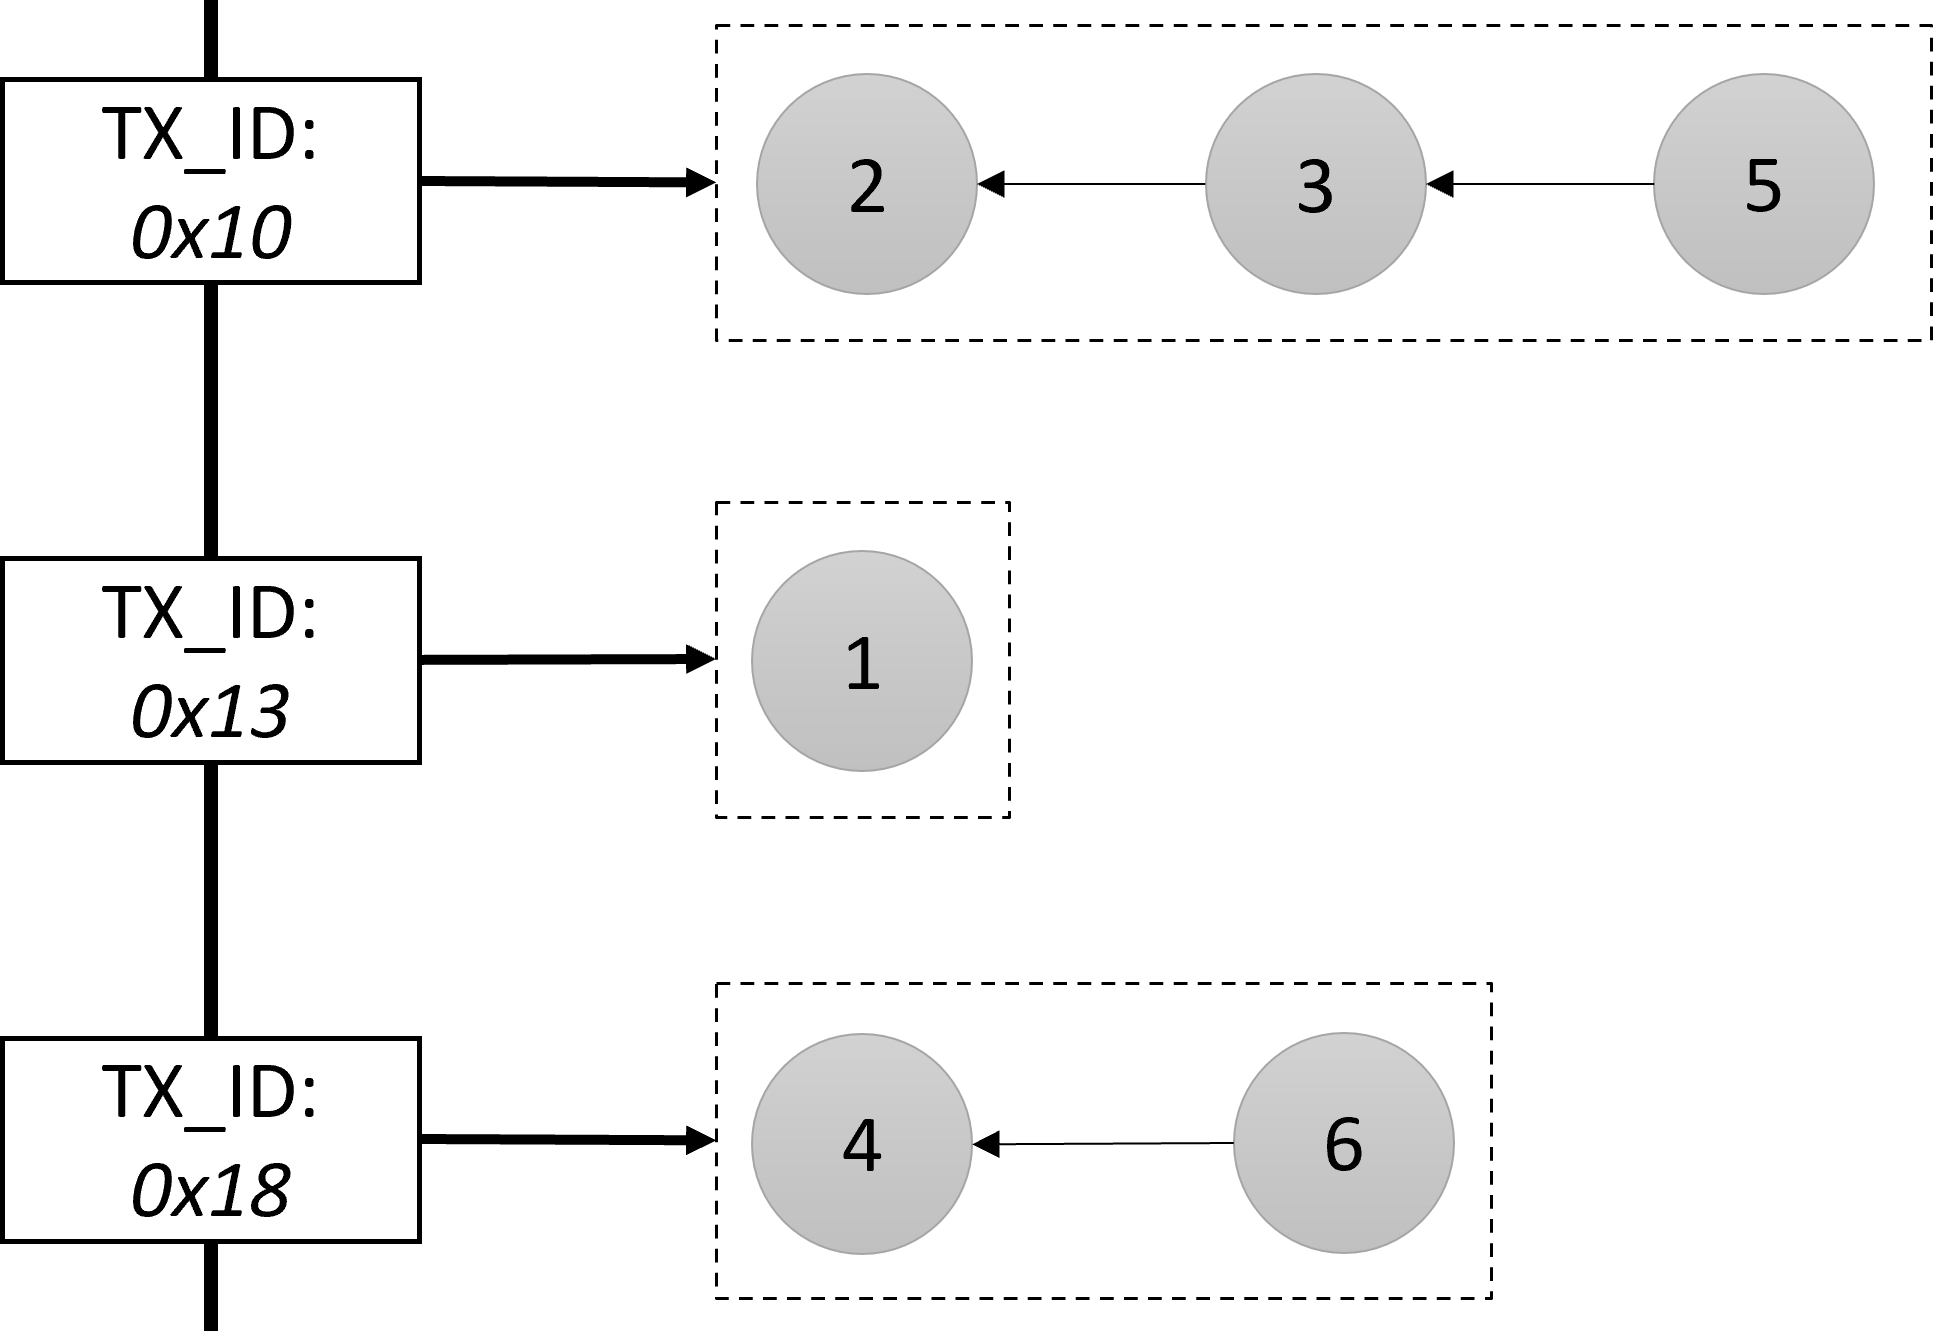
\includegraphics[width=0.7\textwidth]{Figures/store_comparision.png}
    \caption{Execution-Time comparision of a single write-operation on different stores.}
    \label{fig:store_comparision}
\end{figure}

%%%%%%%%%%%%%%%%%%%%%%%%%%%%%%%%%%%%%%%%%%%%%%%%%%%%%%%%%%%%%%%%%%



\subsubsection{TERMINAL 1 vs TERMINAL 50 } 
\begin{figure}[t] 
    \centering 
    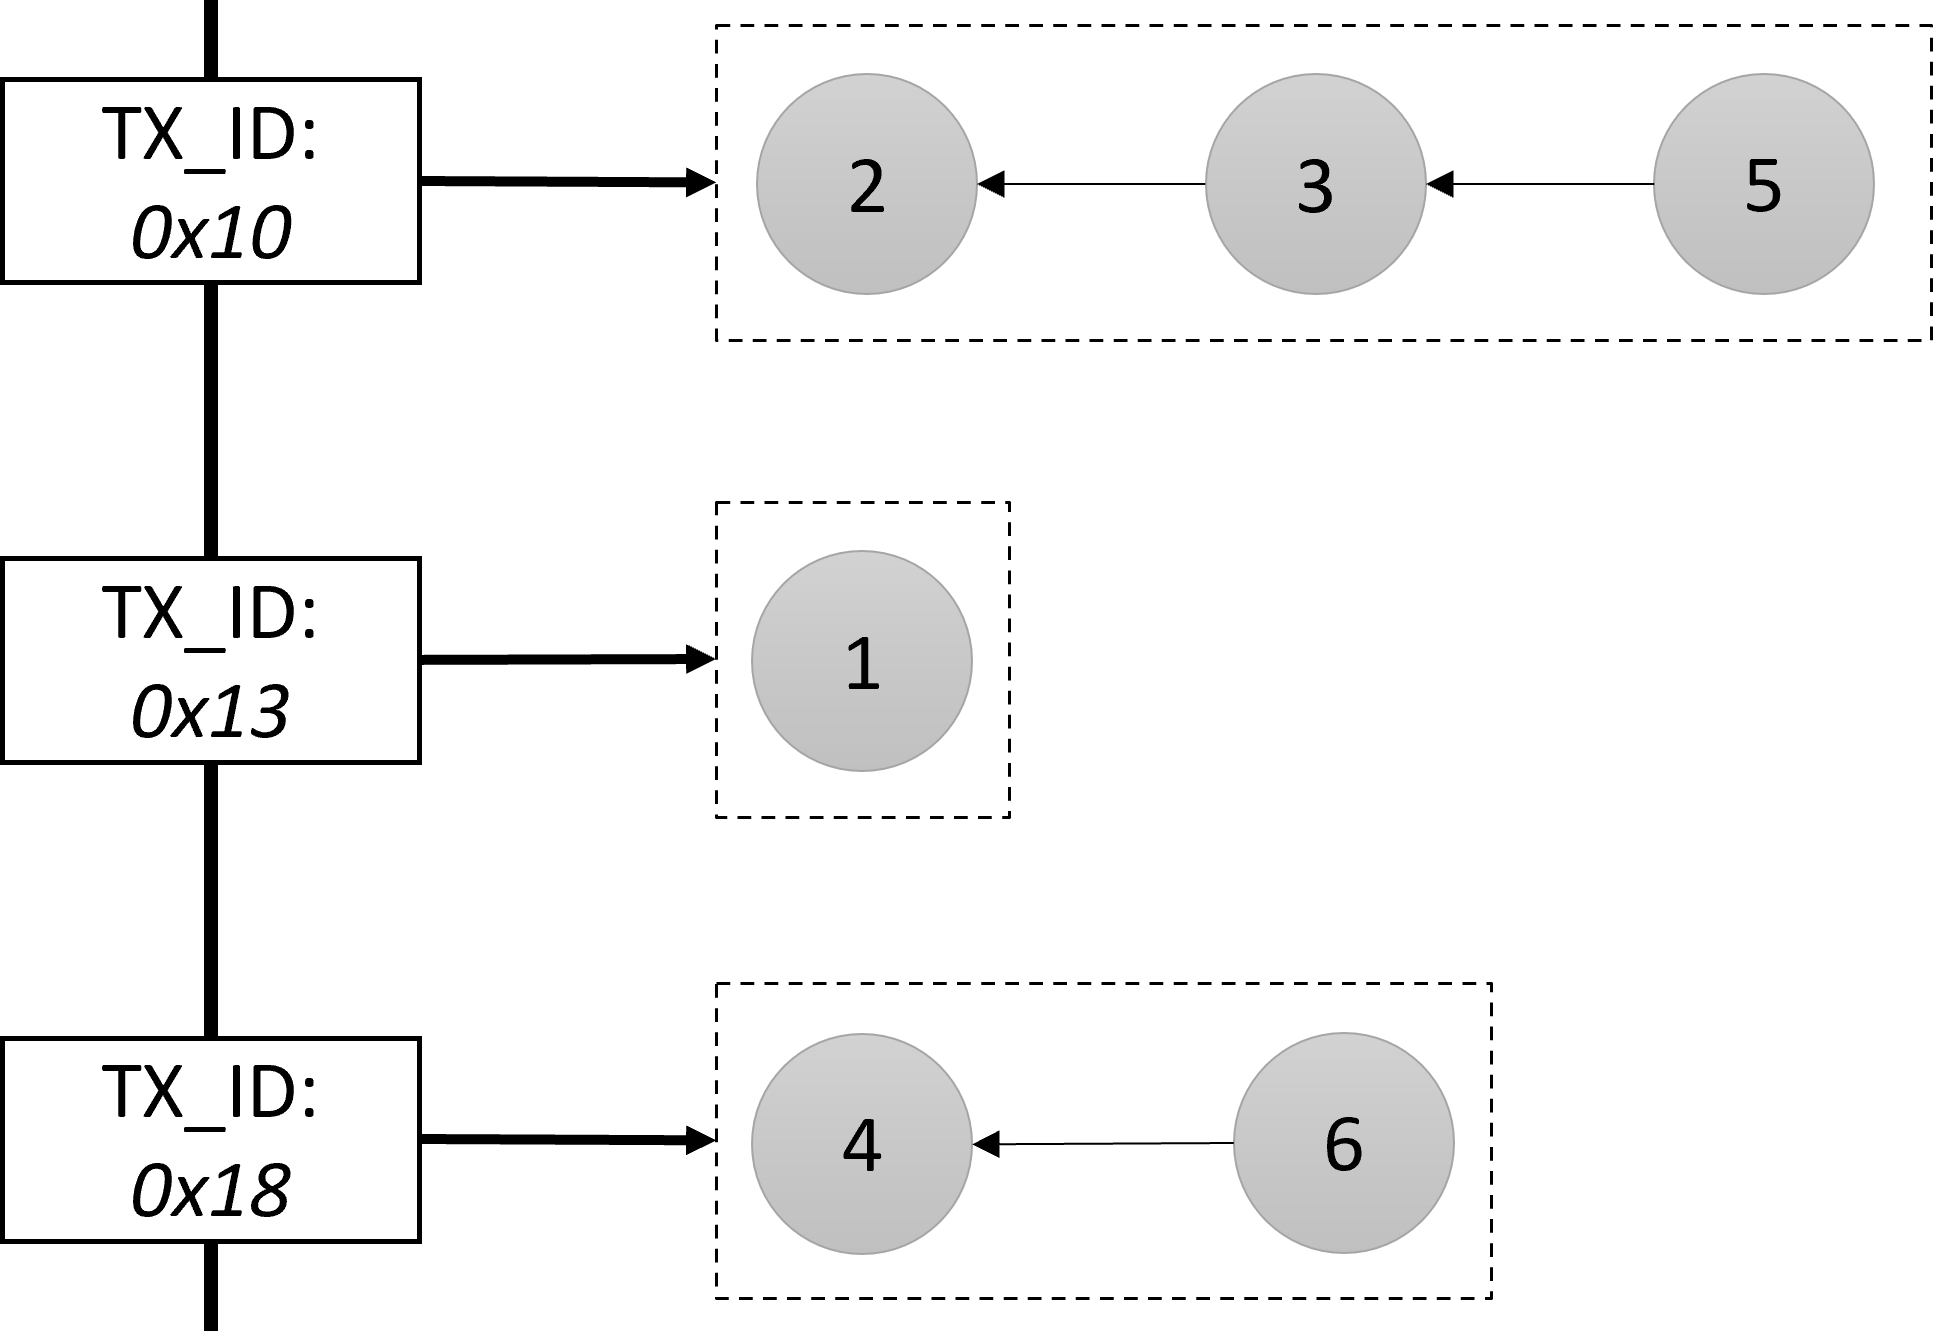
\includegraphics[width=0.7\textwidth]{Figures/store_comparision.png}
    \caption{Execution-Time comparision of a single write-operation on different stores.}
    \label{fig:store_comparision}
\end{figure}

%%%%%%%%%%%%%%%%%%%%%%%%%%%%%%%%%%%%%%%%%%%%%%%%%%%%%%%%%%%%%%%%%%


\subsubsection{PSQL vs HSQL } 
\begin{figure}[t] 
    \centering 
    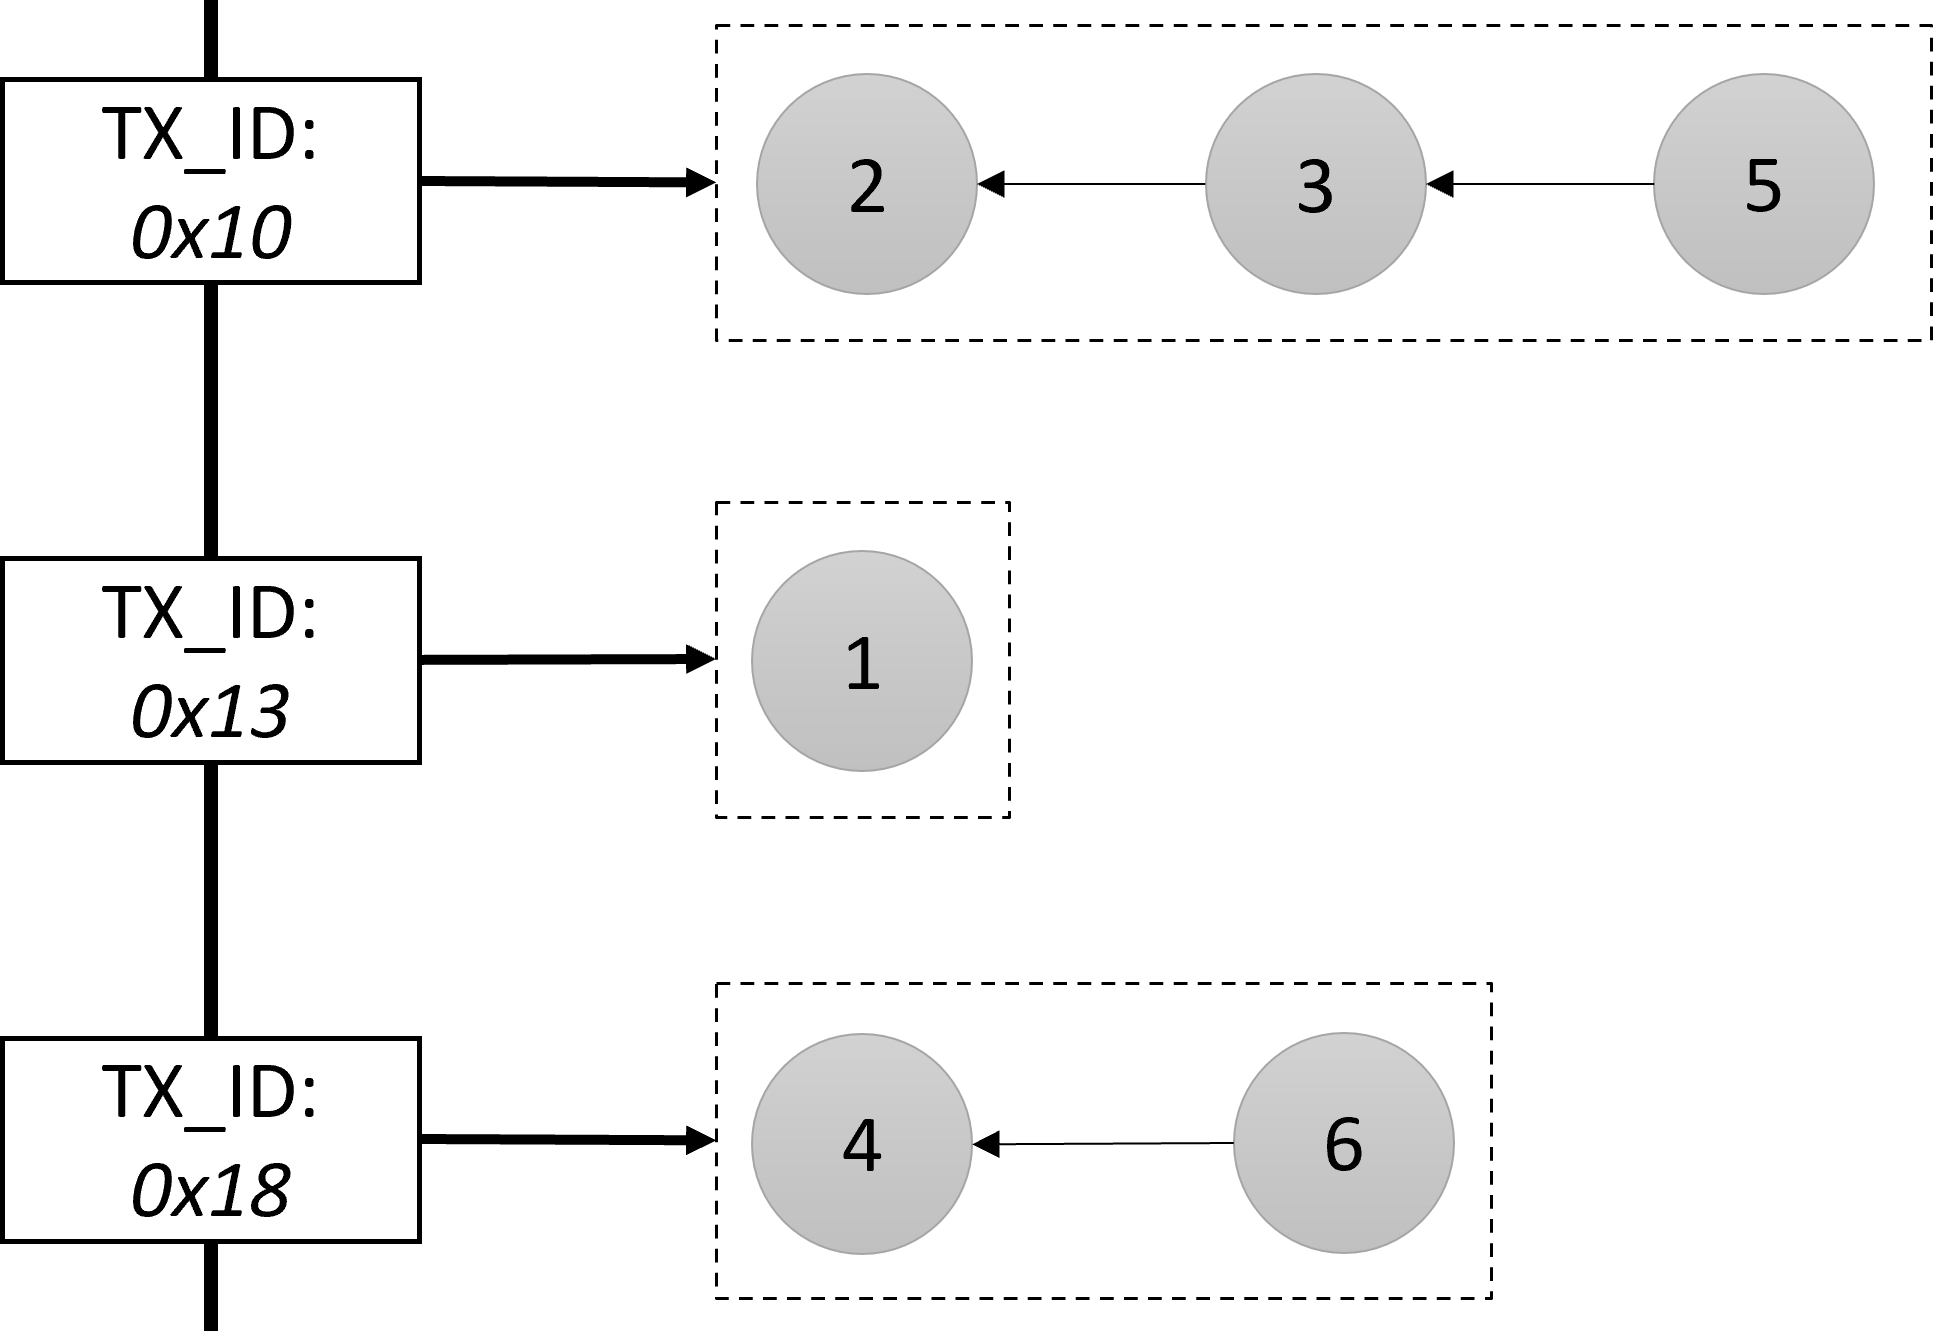
\includegraphics[width=0.7\textwidth]{Figures/store_comparision.png}
    \caption{Execution-Time comparision of a single write-operation on different stores.}
    \label{fig:store_comparision}
\end{figure}

%%%%%%%%%%%%%%%%%%%%%%%%%%%%%%%%%%%%%%%%%%%%%%%%%%%%%%%%%%%%%%%%%%


\subsubsection{Locking } 
\begin{figure}[t] 
    \centering 
    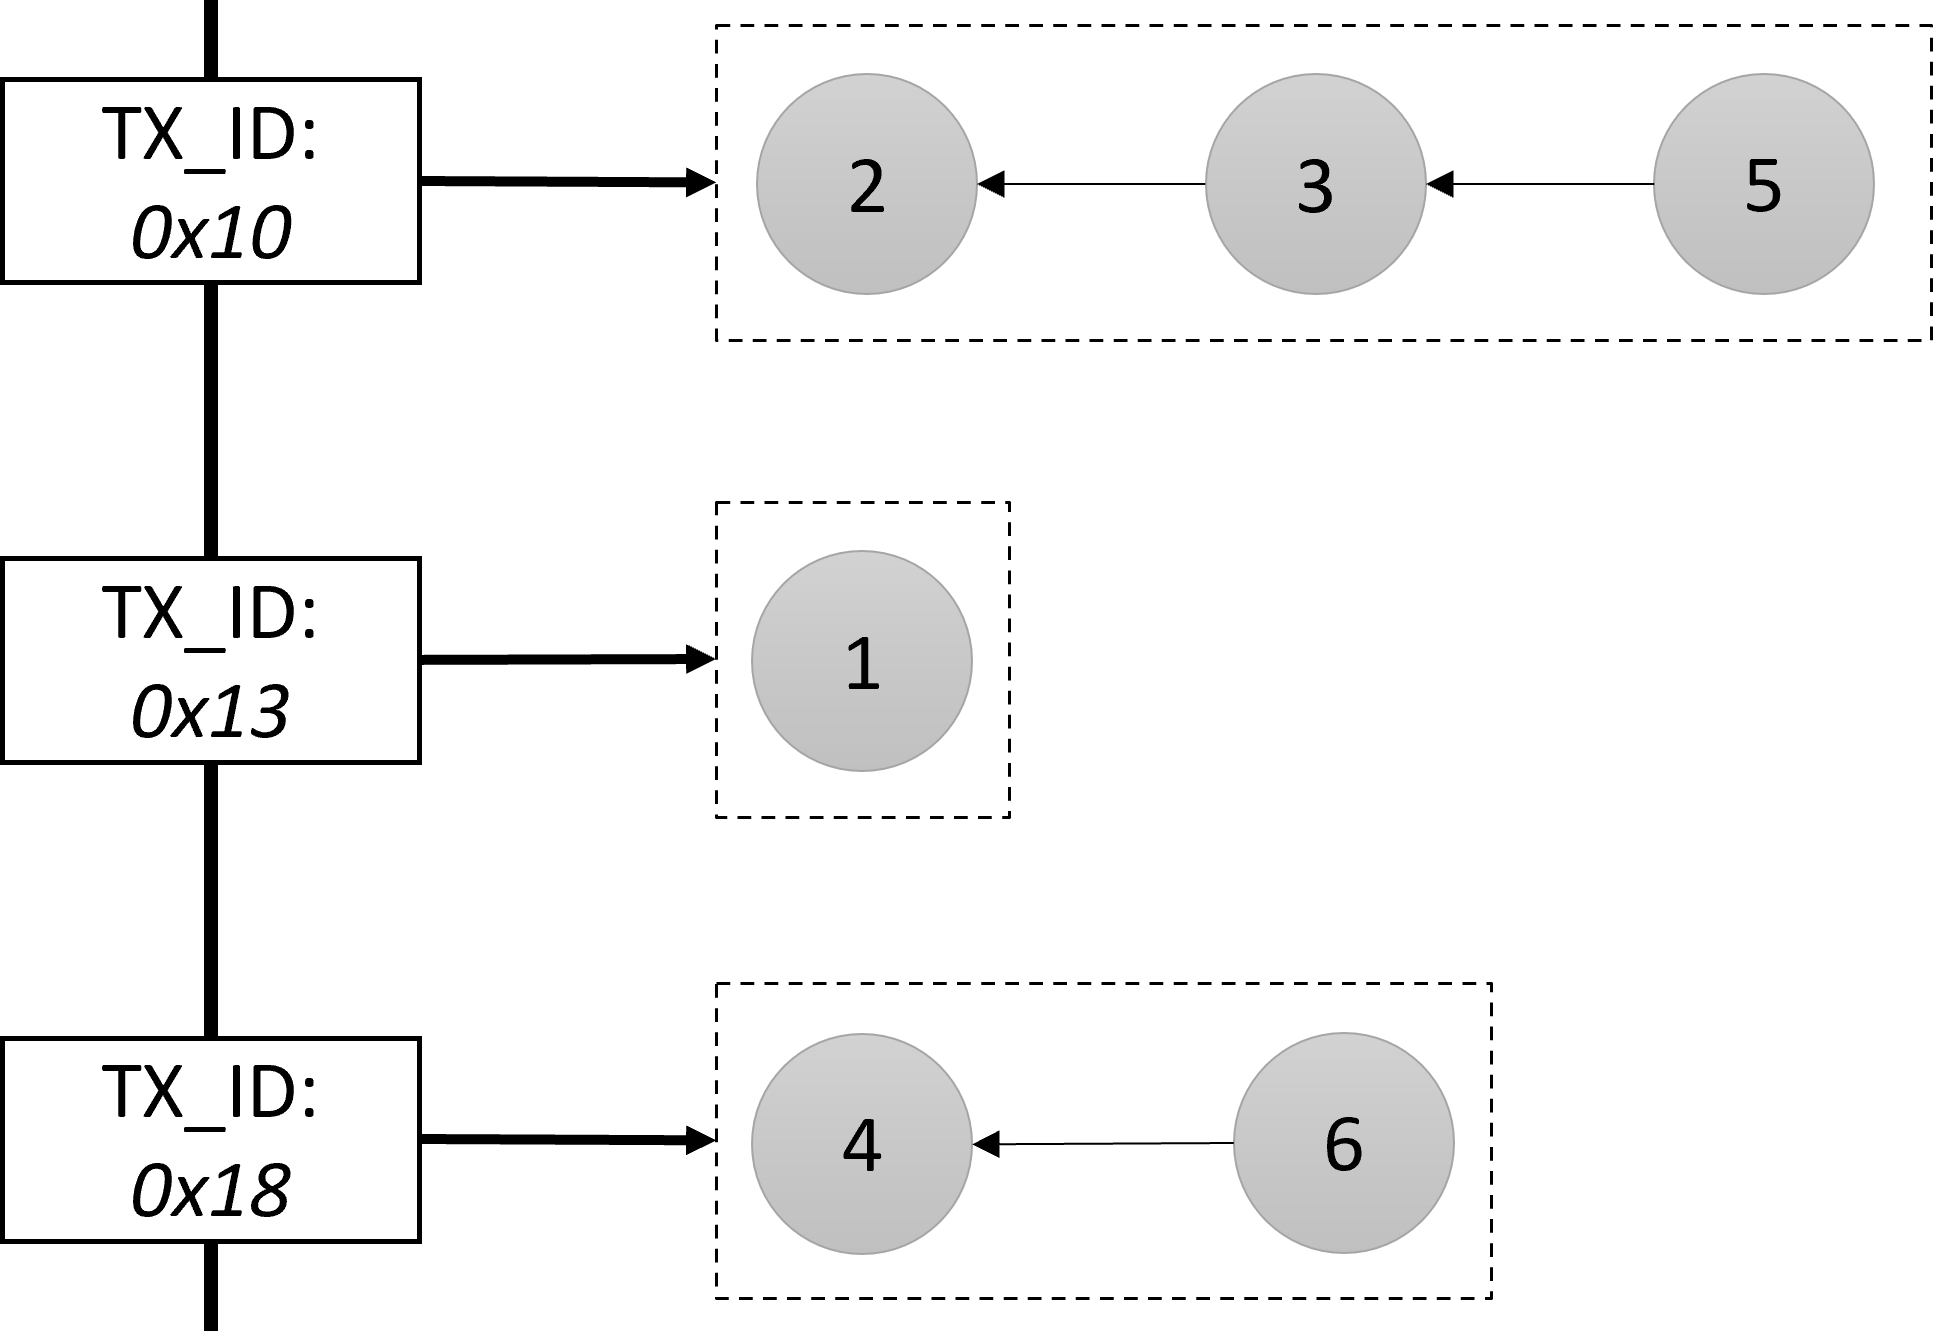
\includegraphics[width=0.7\textwidth]{Figures/store_comparision.png}
    \caption{Execution-Time comparision of a single write-operation on different stores.}
    \label{fig:store_comparision}
\end{figure}

%%%%%%%%%%%%%%%%%%%%%%%%%%%%%%%%%%%%%%%%%%%%%%%%%%%%%%%%%%%%%%%%%%



\subsubsection{Locking } 
\begin{figure}[t] 
    \centering 
    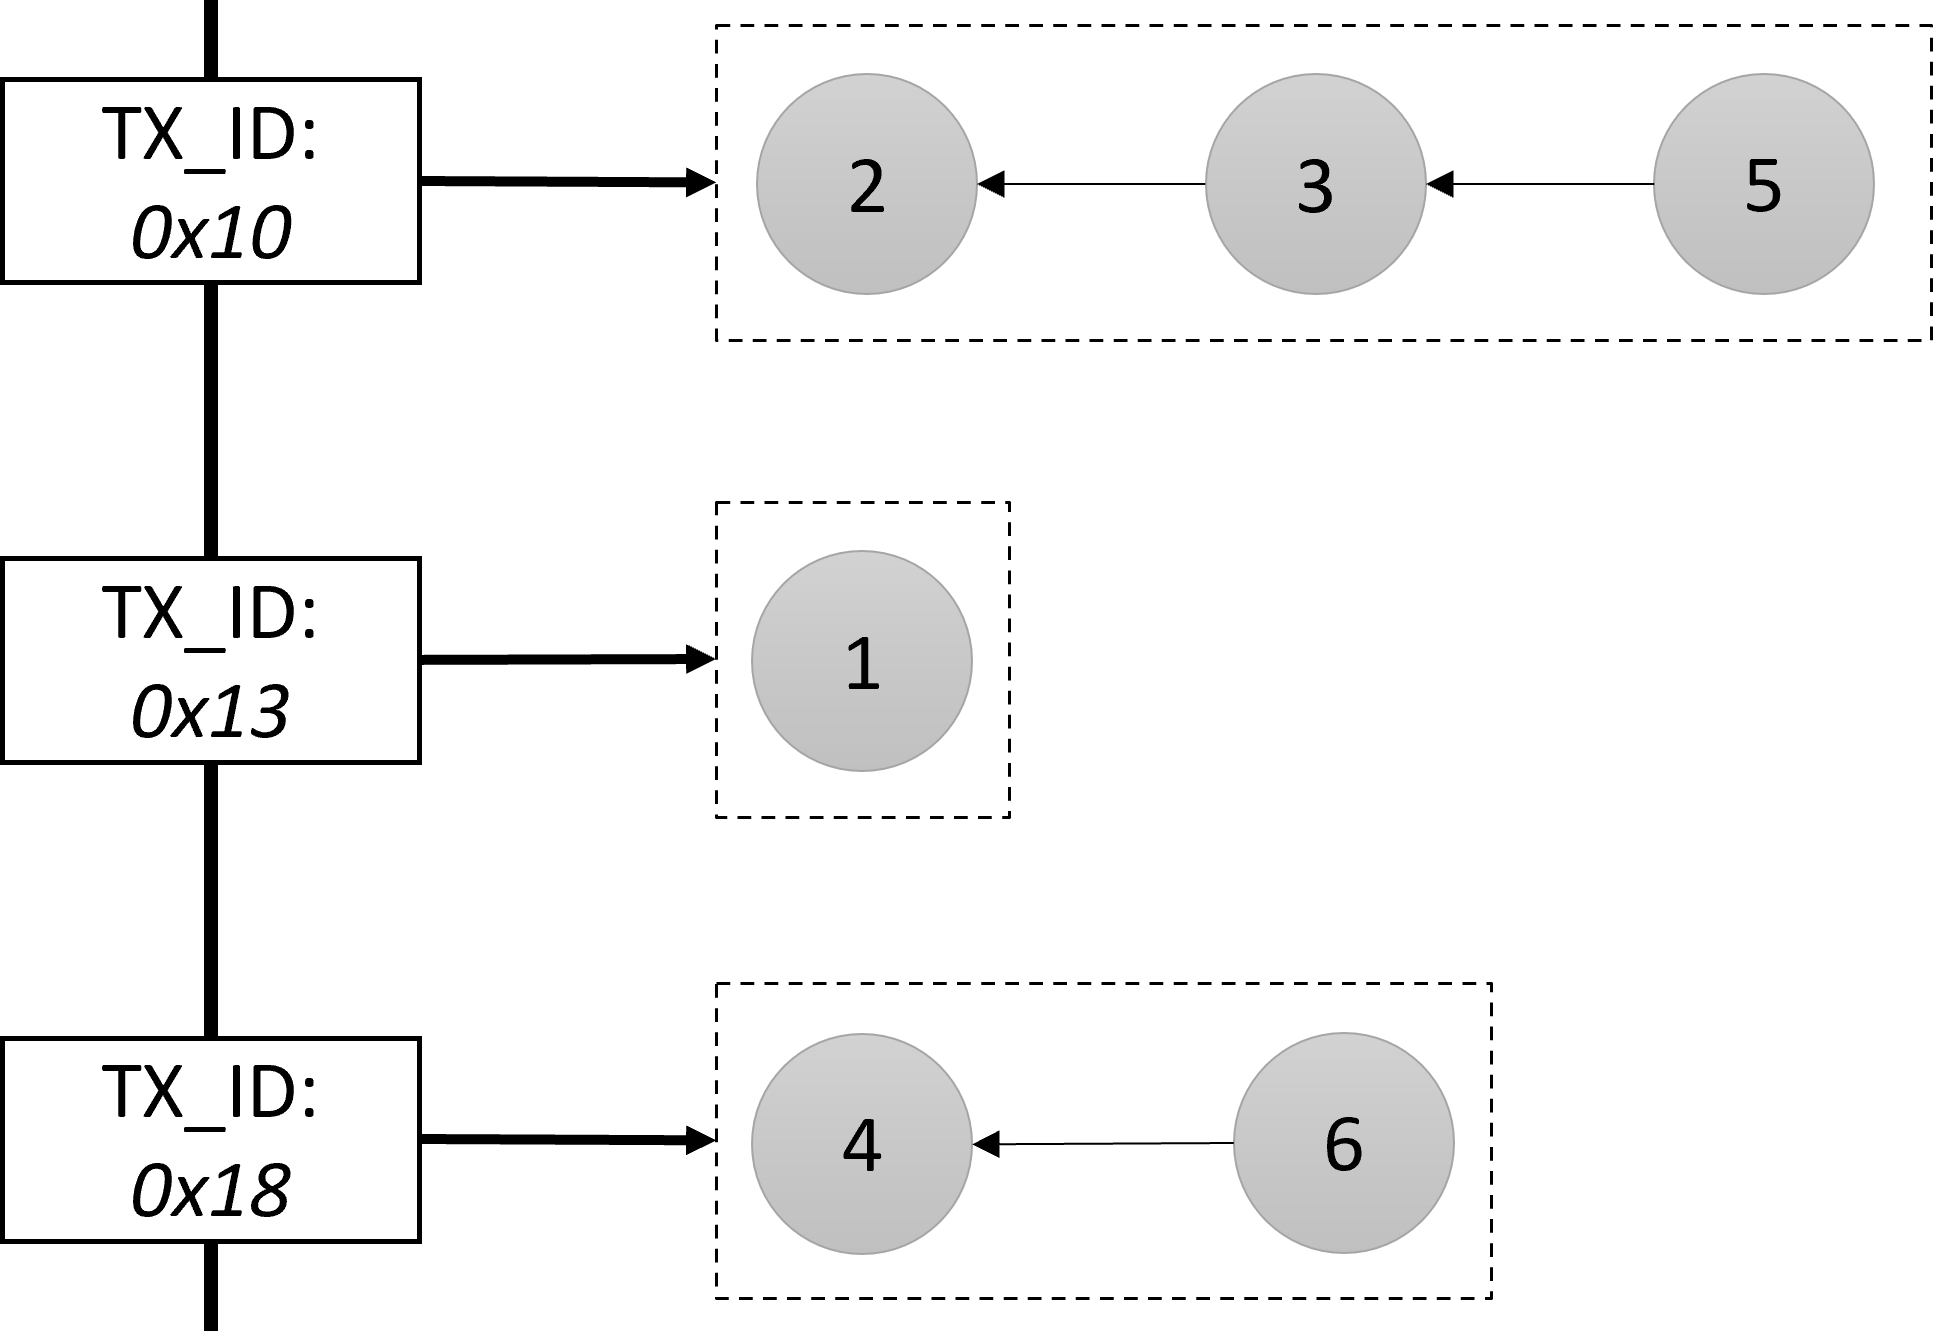
\includegraphics[width=0.7\textwidth]{Figures/store_comparision.png}
    \caption{Execution-Time comparision of a single write-operation on different stores.}
    \label{fig:store_comparision}
\end{figure}

%%%%%%%%%%%%%%%%%%%%%%%%%%%%%%%%%%%%%%%%%%%%%%%%%%%%%%%%%%%%%%%%%%


\subsection{Results}
\label{sec:discussion}

The result generally shows
%%%%%%%%%%%%%%%%%%%%%%%%%%%%%%%%%%%%%%%%%%%%%%%%%%%%%%%%%%%%%%%%%%



